\documentclass[aspectratio=169]{beamer}
\usepackage[deluxe]{luatexja-preset}
\renewcommand{\kanjifamilydefault}{\gtdefault}
\usepackage{minted}
\usepackage{xcolor}
\usepackage{hyperref}
\setbeamertemplate{navigation symbols}{}

\title{テスト駆動開発 ハンズオン \#1}
\author{asuka y}
\date{Aug 21 2022}

\begin{document}

\begin{frame}
  \titlepage
\end{frame}

\section*{INDEX}
\begin{frame}
  \frametitle{テスト駆動揮発ハンズオン \#1}
  \tableofcontents
\end{frame}

\section{テスト駆動開発とは何か}
\subsection{by Wikibedia}
\begin{frame}\frametitle{
    by
    \href{https://ja.wikipedia.org/wiki/\%E3\%83\%86\%E3\%82\%B9\%E3\%83\%88\%E9\%A7\%86\%E5\%8B\%95\%E9\%96\%8B\%E7\%99\%BA}{\underline{Wikibedia}}
  }
  \begin{quotation}
    テスト駆動開発 (てすとくどうかいはつ、英: test-driven development; TDD) とは、プログラム開発手法の一種で、プログラムに必要な各機能について、最初にテストを書き(これをテストファーストと言う)、そのテストが動作する必要最低限な実装をとりあえず行なった後、コードを洗練させる、という短い工程を繰り返すスタイルである。  
    多くのアジャイルソフトウェア開発手法、例えばエクストリーム・プログラミングにおいて強く推奨されている。近年はビヘイビア駆動開発へと発展を遂げている。
  \end{quotation}
\end{frame}

\subsection{認識の間違いからくる現状と課題}
\begin{frame}\frametitle{現状と課題}
  \begin{itemize}
    \item まずは実装してみて後からテストを書こう。
    \item テストを書くことでシステムの品質を担保する。
    \item テストは成果物、カバレッジ100\%です。
    \item テストを何故書くのかを理解されていない。
  \end{itemize}
\end{frame}

\begin{frame}\frametitle{まずは実装してみて後からテストを書こう。}
  テスト駆動開発(TDD)では最初にテストを書く(何故かは後述)。

  しかし現実問題として「時間がないのでまずは実装をしたい、テストは後回しだ!」といったことは多々起こってる。
  \begin{figure}
    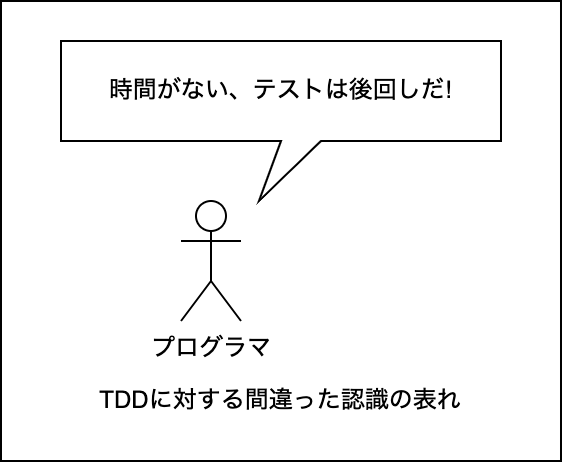
\includegraphics[height=5cm]{asset/bad_programmer.png}
  \end{figure}
  この発想自体がTDDに対して間違った認識をしてしまっていることの表れである。
\end{frame}

\begin{frame}\frametitle{テスト後回しにすることによって起きる悲劇}
  テストを後回しにすることの最大の悲劇は、全ての実装を終えた後にテストを書こうとしてテストを書けないことに気がつくことである。
  \begin{figure}
    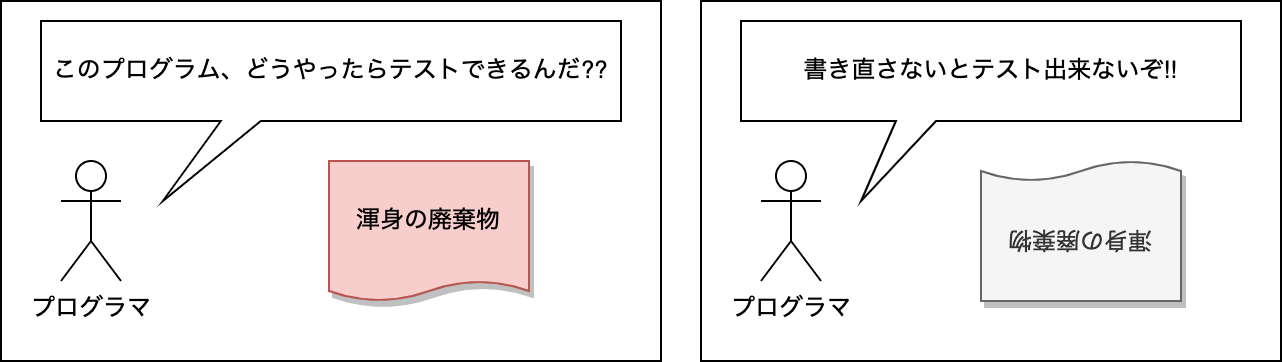
\includegraphics[height=4cm]{asset/gabage_code.png}
  \end{figure}
  そしてテストを書くために今までのコードを全て書き直すことになる。
\end{frame}

\begin{frame}\frametitle{テストを書くことで品質を担保する。}
  これもTDDに対する認識の間違い。
  TDDの結果として品質の良いプログラムが出来上がることがあったとしても、
  TDDは品質を担保することを目的としていない。
\end{frame}

\begin{frame}[fragile]\frametitle{テストは成果物、カバレッジ100\%です。}
  これはそもそもテストを理解していないパターンが多い。
  カバレッジはテストを書く時の目安になることはあっても、カバレッジによってテストの正しさが証明されることはない。
\end{frame}

\begin{frame}[fragile]\frametitle{テストを何故書くのかを理解されていない。}
  このテストはこの機能が正しいことをテストしていないよね(よくあるパターン)
  \begin{minted}[fontsize=\scriptsize]{php}
    <?php
    /**
     * テスト対象
     */
    class Foo {
      function is_enable(): bool {
        // 多くの依存関係
        return $is_inable;
      }
    }

    /**
     * Fooをテストするためのモック
     */
    class MockFoo extends Foo {
      function is_enable(): bool {
        return $this->enable;
      }
    }
  \end{minted}
\end{frame}

\subsection{テスト駆動開発とは何か}
\begin{frame}\frametitle{テスト駆動開発とは何か}
  {\small \color[gray]{0.5} テスト駆動開発「まえがき」}
  \begin{quotation}
    「動作するきれいなコード」。Ron Jeffries のこの簡潔な言葉が、テスト駆動開発(TDD)のゴールだ。
    動作するきれいなコードはあらゆる意味で価値がある。
  \end{quotation}

  {\small \color[gray]{0.5} テスト駆動開発「本文」}
  \begin{quotation}
    TDDはテスト技法ではない...TDDは分析技法であり、設計技法であり、実際には開発の全てのアクティビティを構造化する技法なのだ。
  \end{quotation}

  \vspace{1\baselineskip}
  完全に理解した。
\end{frame}

\subsection{ハンズオンをやる目的}
\begin{frame}\frametitle{ハンズオンをやる目的}
  チームメンバーの誰もがユニットテストを書いたことがなかった時、
  新しいサービスを作るときに新しいプロダクトをTDDで進めようと踏み切れるだろうか?

  \vspace{1\baselineskip}
  TDDは開発における設計技法であるということを理解しないと
  永遠に実装終えた後のテストで苦しむことになる。
  ハンズオンを通してTDDを実践することで、TDDを採用する際の迷いを取り除くことが目的。
\end{frame}

\section{テスト駆動開発の進め方}
\begin{frame}\frametitle{テスト駆動開発の進め方}
  {\small \color[gray]{0.5} テスト駆動開発「第1部」}
  \begin{enumerate}
    \item まずはテストを1つ書く
    \item 全てのテストを走らせ、新しいテストの失敗を確認する
    \item 小さな変更を行う
    \item 全てのテストを走らせ、全て成功することを確認する
    \item リファクタリングを行なって重複を排除する
  \end{enumerate}

  \vspace{1\baselineskip}
  ここに書かれていることはベストプラクティスと捉えてもらえると良い。
  テスト駆動開発はこのサイクルを回して開発を進めることになる。
\end{frame}

\subsection{まずはテストを1つ書く}
\begin{frame}\frametitle{まずはテストを1つ書く}
\end{frame}

\subsection{全てのテストを走らせ、新しいテストの失敗を確認する}
\begin{frame}\frametitle{全てのテストを走らせ、新しいテストの失敗を確認する}
\end{frame}

\subsection{小さな変更を行う}
\begin{frame}\frametitle{小さな変更を行う}
\end{frame}

\subsection{全てのテストを走らせ、全て成功することを確認する}
\begin{frame}\frametitle{全てのテストを走らせ、全て成功することを確認する}
\end{frame}

\subsection{リファクタリングを行なって重複を排除する}
\begin{frame}\frametitle{リファクタリングを行なって重複を排除する}
\end{frame}

\section{ハンズオン}
\subsection{フィボナッチ数列}
\begin{frame}\frametitle{ハンズオン: フィボナッチ数列}
\end{frame}

\subsection{逆ポーランド電卓}
\begin{frame}\frametitle{ハンズオン: 逆ポーランド電卓}
\end{frame}

\subsection{RESTful API}
\begin{frame}\frametitle{ハンズオン: RESTful API}
\end{frame}

\end{document}
